
% \section{Initiation aux langages de description matérielle : VHDL}

\begin{frame}{HDL : Hardware description language}
  \begin{itemize}
    \item Les HDL permettent de \textbf{décrire} des systèmes.
    \begin{itemize}
      \item ...de le même manière que \texttt{html} permet de décrire le contenu d'une page web.
    \end{itemize}
    \item Ils sont donc très différents des langages de programmation classiques.
  \end{itemize}

  A titre d'exemple, nous donnons ici un code d'un HDL très important en Electronique {\it analogique} : \textbf{Spice}.
  Spice permet de décrire comment les composants usuels (résistance, capacité, inductance) sont interconnectés.
  Le simulateur Spice permet de rendre compte du comportement du circuit.
  \textbf{Nous allons procéder de même avec VHDL}, mais à plus haut niveau.
  \begin{figure}[h!]
    \centering
    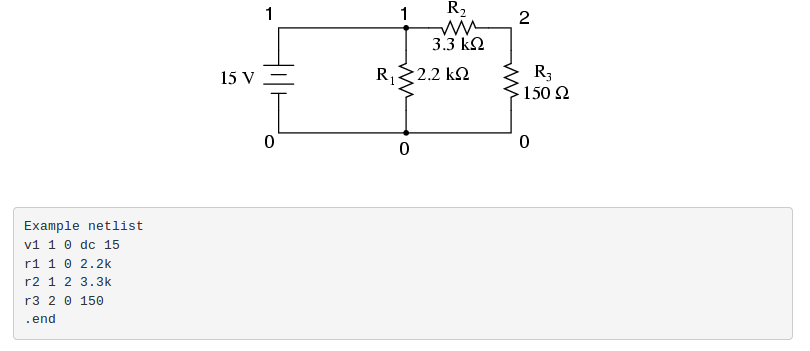
\includegraphics[scale=0.30]{./images/spice.png}
  \end{figure}
\end{frame}

\begin{frame}{Historique de VHDL}
  \begin{itemize}
    \item VHDL est l'acronyme de : VHSIC Hardware Description Language.
    \begin{itemize}
      \item VHSIC : Very High Speed Integrated Circuit
    \end{itemize}
    \item VHDL a été commandé par le Département à la Défense Américaine (DoD).
    \item Sa syntaxe s'inspire fortement d'\textbf{ADA}, très utilisé en \textit{logiciel} dans les années 80.
    \item VHDL est fortement et explicitement \textbf{typé}.
    \item Le but initial était de permettre aux acteurs de la Silicon Valley de seulement échanger des informations/designs de manière cohérente.
    \item Son concurrent direct est le langage \textbf{Verilog}.
    \item VHDL est un langage \textit{réputé difficile}. Il parle de :
    \begin{itemize}
      \item structures qui opèrent en parallèle
      \item signaux
      \item deux formes de temps
    \end{itemize}
  \end{itemize}

  Ces langages sont standardisés par l'IEEE. Plusieurs versions pour VHDL : 87,\textbf{93},08 notamment.
\end{frame}

\begin{frame}{VHDL : Simulation \& Synthèse}
  \begin{columns}
    \begin{column}{0.5\textwidth}
      VHDL est utilisé pour deux activités différentes :
      \begin{itemize}
        \item La \textbf{simulation} : vérification fonctionnelle sur PC, du bon fonctionnement du système décrit.
        \item La \textbf{synthèse} : la génération automatique du système à partir des descriptions.
        \begin{itemize}
          \item Ces descriptions sont de plus en plus abstraites.
          \item On se limitera essentiellement dans ce cours à décrire le circuit en terme d'équations logiques.
          \item Le niveau directement plus abstrait est le niveau RTL.
        \end{itemize}
      \end{itemize}
      \begin{alertblock}{Flot de conception}
        \begin{itemize}
          \item L'ingénierie des systèmes numériques requiert une organisation méticuleuse.
          \item Autant techniquement qu'humainement.
        \end{itemize}
      \end{alertblock}
    \end{column}
    \begin{column}{0.5\textwidth}
      \begin{center}
        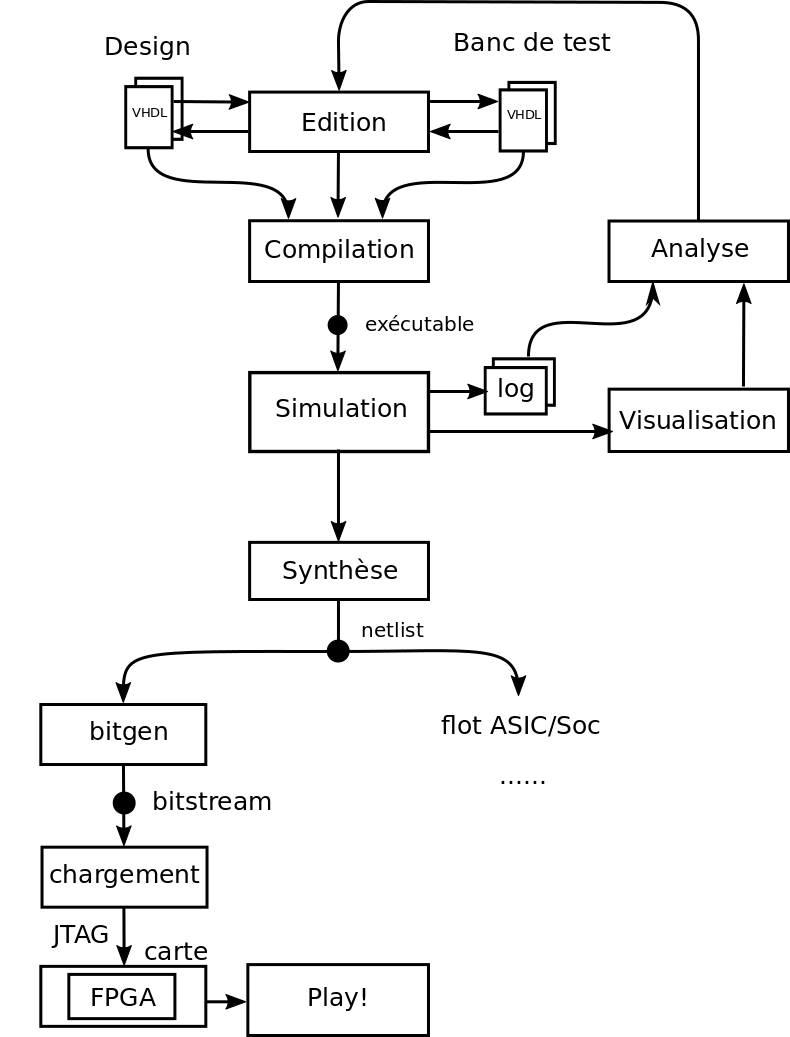
\includegraphics[scale=0.18]{./images/conception_generale.png}
      \end{center}
    \end{column}
  \end{columns}
\end{frame}

% \begin{frame}{Flot général}
% \begin{columns}
%   \begin{column}{0.5\textwidth}
%   \end{column}
%   \begin{column}{0.5\textwidth}
%   \end{column}
% \end{columns}
% \end{frame}

\begin{frame}{Survol de la Simulation VHDL}
  \begin{columns}
    \begin{column}{0.45\textwidth}
      La simulation, réalisée sur PC :
      \begin{itemize}
        \item Repose sur un \textbf{mécanisme d'échéancier} :
        \begin{itemize}
          \item Event-driven simulator.
          \item Image d'une \textit{to-do list}.
        \end{itemize}
        \item Le temps est incrémenté petit-à-petit :
        \begin{itemize}
          \item \textbf{Temps physique} simulé
          \item \textbf{Temps causal} : {\it delta delay/cycles}. Pas infinitésimaux de propagation.
        \end{itemize}
        \item Le simulateur préserve la \textbf{causalité} entre signaux.
        \item C'est une tâche non-triviale pour un programme (simulateur) qui s'exécute sur un ordinateur séquentiel.
      \end{itemize}
    \end{column}
    \begin{column}{0.55\textwidth}
      \begin{center}
        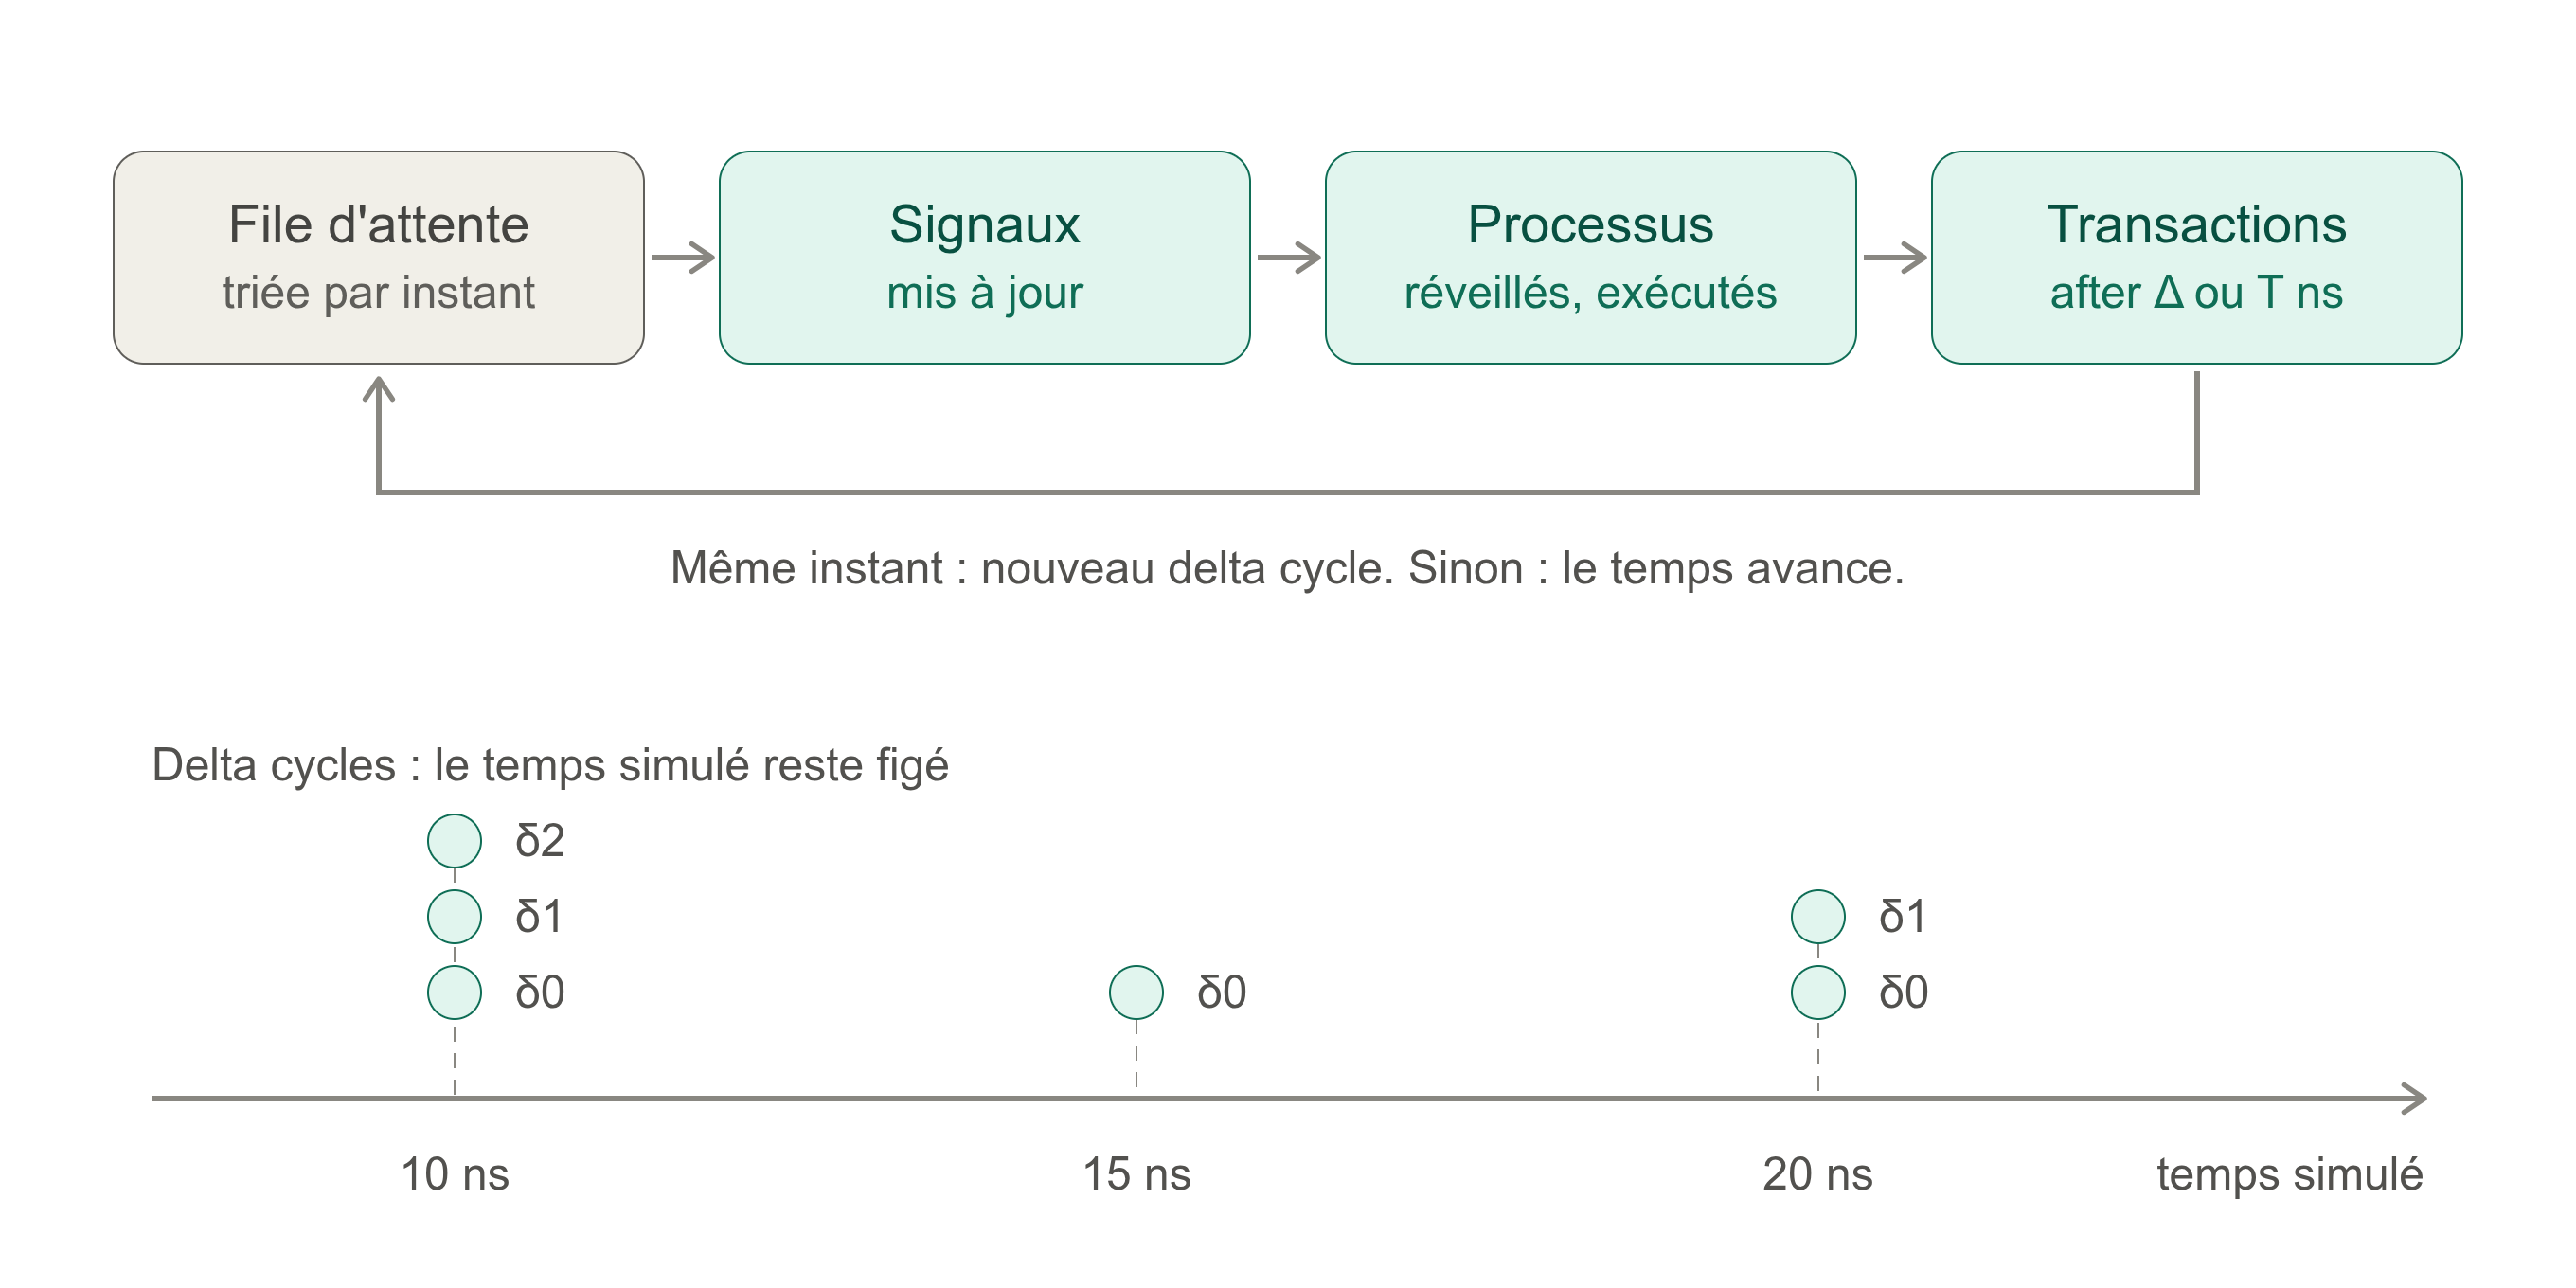
\includegraphics[scale=0.09]{./images/simulation_evenements_discrets_vhdl.png}
      \end{center}
    \end{column}
  \end{columns}
\end{frame}

\begin{frame}{La synthèse logique : du RTL à la netlist mappée}
  \begin{columns}[T,onlytextwidth]

  % ---------- Colonne gauche : explication ----------
  \begin{column}{0.46\textwidth}
    \small
    \textbf{Définition}\\[2pt]
    Transformer une description RTL (VHDL synthétisable) en une
    \emph{netlist} de cellules d'une technologie cible (FPGA ou ASIC).

    \vspace{6pt}
    \textbf{Étapes principales}
    \begin{enumerate}
      \item \textbf{Élaboration} : analyse du code, résolution de la
            hiérarchie, inférence de logique combinatoire et de registres.
      \item \textbf{Optimisation} : minimisation booléenne, partage de
            sous-expressions, suppression de la logique inutile.
      \item \textbf{Mapping technologique} : recouvrement du graphe de portes
            par les cellules du vendeur (LUT, bascules, cellules standard).
    \end{enumerate}

    \vspace{4pt}
    Le mapping est piloté par la \textbf{bibliothèque vendeur} et par les
    \textbf{contraintes} (fréquence, surface, puissance).

    \vspace{4pt}
    \textbf{Résultat} : une netlist mappée, prête pour le placement-routage.
  \end{column}

  % ---------- Colonne droite : schéma ----------
  \begin{column}{0.52\textwidth}
    \centering
    \begin{tikzpicture}[
        scale=0.88, every node/.style={transform shape},
        gbox/.style={draw=gray!70, fill=gray!15, rounded corners=3pt, line width=0.4pt},
        tbox/.style={draw=teal!80!black, fill=teal!15, rounded corners=3pt, line width=0.4pt},
        cell/.style={draw=gray!80, fill=white, rounded corners=1.5pt, line width=0.4pt,
                     font=\scriptsize, inner sep=1pt},
        arr/.style={-{Stealth[length=1.8mm]}, line width=0.7pt},
        wire/.style={line width=0.5pt},
        lbl/.style={font=\footnotesize\bfseries, align=right}
      ]
      % --- RTL ---
      \draw[gbox] (0,0) rectangle (4.2,-1.2);
      \node[font=\footnotesize\bfseries] at (2.1,-0.32) {RTL (VHDL)};
      \node[font=\footnotesize\ttfamily] at (2.1,-0.82) {y <= (a and b) or c;};

      % --- flèche 1 ---
      \draw[arr] (2.1,-1.2) -- (2.1,-2.1);
      \node[lbl, anchor=east] at (1.95,-1.65) {Élaboration};

      % --- Netlist générique ---
      \draw[gbox] (0,-2.1) rectangle (4.2,-4.3);
      \node[font=\footnotesize\bfseries] at (2.1,-2.42) {Netlist générique};
      \node[font=\scriptsize] at (2.1,-2.74) {portes et bascules};
      \node[cell, minimum width=0.8cm, minimum height=0.5cm] (and) at (1.3,-3.35) {AND};
      \node[cell, minimum width=0.8cm, minimum height=0.5cm] (or)  at (2.9,-3.35) {OR};
      \draw[wire] (0.65,-3.23) -- (and.west |- 0,-3.23);
      \draw[wire] (0.65,-3.47) -- (and.west |- 0,-3.47);
      \node[font=\scriptsize] at (0.4,-3.23) {a};
      \node[font=\scriptsize] at (0.4,-3.47) {b};
      \draw[arr] (and.east) -- (or.west);
      \draw[wire] (or.east) -- (3.65,-3.35);
      \node[font=\scriptsize] at (3.85,-3.35) {y};
      \draw[arr] (2.9,-3.98) -- (or.south);
      \node[font=\scriptsize] at (2.9,-4.12) {c};

      % --- flèche 2 ---
      \draw[arr] (2.1,-4.3) -- (2.1,-5.2);
      \node[lbl, anchor=east, text width=1.8cm] at (1.95,-4.75)
           {Optimisation\\+ mapping};

      % --- Netlist mappée ---
      \draw[tbox] (0,-5.2) rectangle (4.2,-7.3);
      \node[font=\footnotesize\bfseries] at (2.1,-5.52) {Netlist mappée};
      \node[font=\scriptsize] at (2.1,-5.84) {cellules du vendeur};
      \node[cell, minimum width=1.2cm, minimum height=0.9cm, font=\footnotesize\bfseries]
           (lut) at (2.1,-6.55) {LUT3};
      \foreach \yy/\n in {-6.3/a,-6.55/b,-6.8/c}{
        \draw[wire] (0.85,\yy) -- (lut.west |- 0,\yy);
        \node[font=\scriptsize] at (0.6,\yy) {\n};
      }
      \draw[wire] (lut.east) -- (3.35,-6.55);
      \node[font=\scriptsize] at (3.6,-6.55) {y};

      % --- Bibliothèque vendeur ---
      \draw[tbox] (4.5,-3.85) rectangle (6.7,-5.65);
      \node[align=center, font=\footnotesize] at (5.6,-4.75)
           {\textbf{Bibliothèque}\\\textbf{vendeur}\\[1pt]{\scriptsize cellules, timing,}\\{\scriptsize contraintes}};
      \draw[arr] (4.5,-4.75) -- (2.15,-4.75);
    \end{tikzpicture}
  \end{column}

  \end{columns}
\end{frame}

\begin{frame}{Survol de la Synthèse VHDL}
  \begin{itemize}
    \item La synthèse, réalisée sur PC, permet d'obtenir un circuit (optimisé) à partir d'une description.
    \item Seul un sous-ensemble du langage est "synthétisable", mais il est très large.
    \item Le résultat est fourni sous un format de graphe précisant toutes les interconnexions : "netlist"
    \item Dans le cas de la synthèse sur FPGA, cette netlist est ensuite transformée en \textbf{bitstream}.
  \end{itemize}
  \includegraphics[scale=0.5]{Schematic.pdf}
\end{frame}

%\frame[plain]{\includegraphics[width=\textwidth]{Schematic.pdf}}

\begin{frame}{Structure globale d'une description VHDL}
  \begin{columns}
    \begin{column}{0.4\textwidth}
      En première approche, on peut proposer la structure de fichier suivante :
      \begin{itemize}
        \item Déclaration des bibliothèques et packages utilisés : \textbf{library}...,\textbf{use}...
        \item Déclaration des entrées-sorties du circuit : \textbf{entity}
        \item Déclaration de l'intérieur du circuit : \textbf{architecture}
      \end{itemize}
      \begin{alertblock}{Le monde du parallélisme}
        \begin{itemize}
          \item Entre le \texttt{begin...end} de l'\texttt{architecture}
          \item \textbf{ordre indifférent} des "instructions"...
          \item ...ou plutôt des \textbf{déclarations}.
        \end{itemize}
      \end{alertblock}
    \end{column}
    \begin{column}{0.6\textwidth}
      \begin{figure}[h]
        \centering
        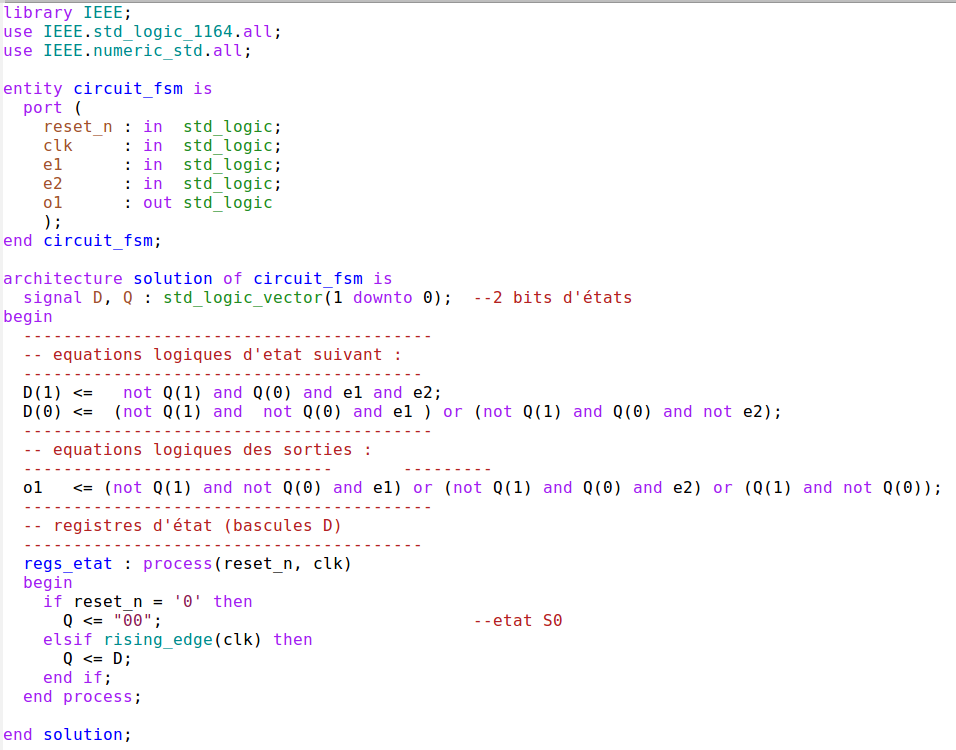
\includegraphics[scale=0.25]{./images/vhdl_1.png}
        %\caption{Vending machine et son environnement}
      \end{figure}
    \end{column}
  \end{columns}
\end{frame}


\begin{frame}{Netlist : après synthèse}
  \begin{columns}
    \begin{column}{0.45\textwidth}
      \begin{figure}[h]
        \centering
        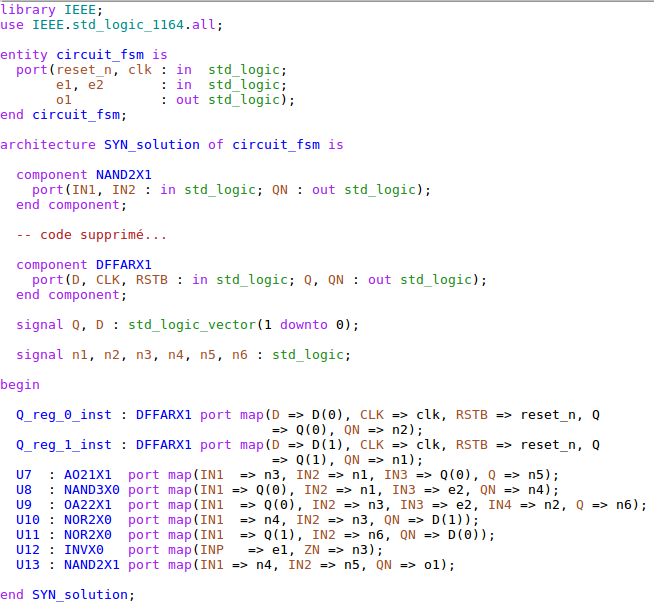
\includegraphics[scale=0.3]{./images/netlist.png}
      \end{figure}
    \end{column}
    \begin{column}{0.55\textwidth}
      \begin{figure}[h]
        \centering
        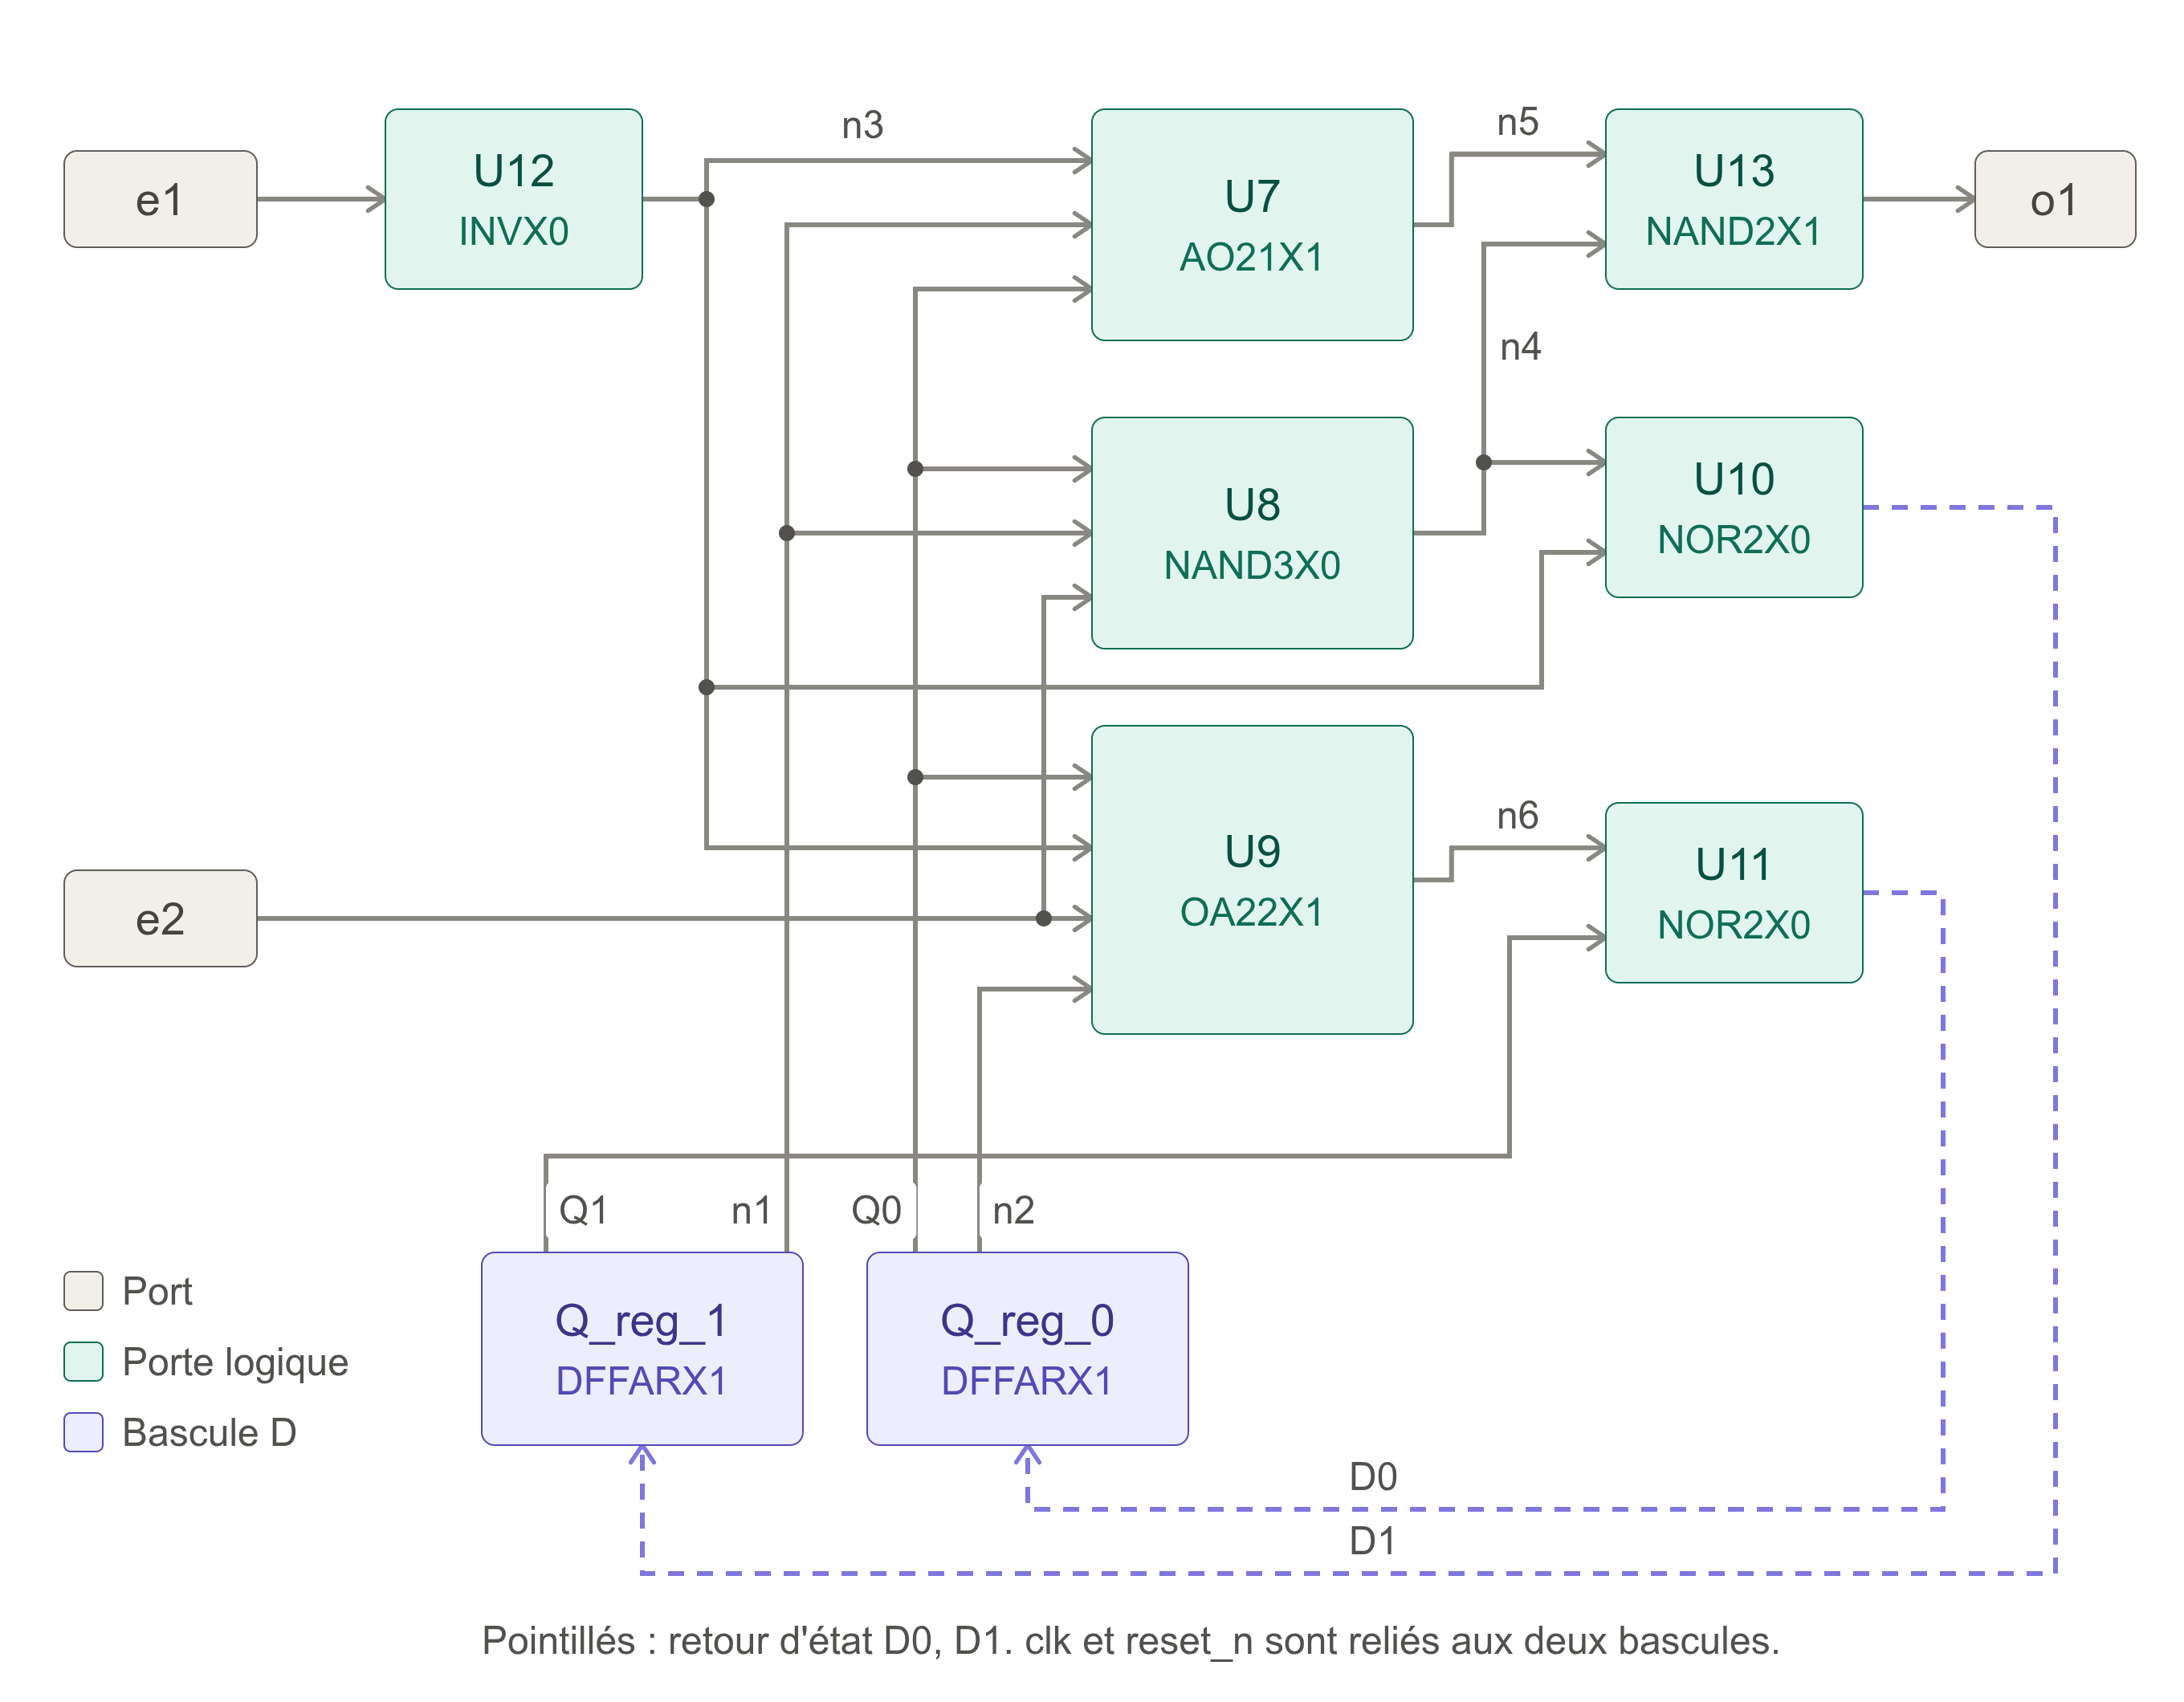
\includegraphics[scale=0.09]{./images/netlist_circuit_fsm_graphe.png}
      \end{figure}
    \end{column}
  \end{columns}
\end{frame}


\begin{frame}{Notion d'entité}
\begin{columns}
  \begin{column}{0.4\textwidth}
    L'\textbf{entity} est la \textbf{vue extérieure} d'un composant.
    \begin{itemize}
      \item Nom du composant
      \item Liste de ports :
      \begin{itemize}
        \item Entrées : \boxed{nom : \textbf{in } type;}
        \item Sorties : \boxed{nom : \textbf{out } type;}
        \item Il est possible de déclarer plusieurs ports comme ceci : \boxed{n1,n2,n3 : \textbf{out } type;}
      \end{itemize}
    \end{itemize}
  \end{column}
  \begin{column}{0.6\textwidth}
    \begin{center}
      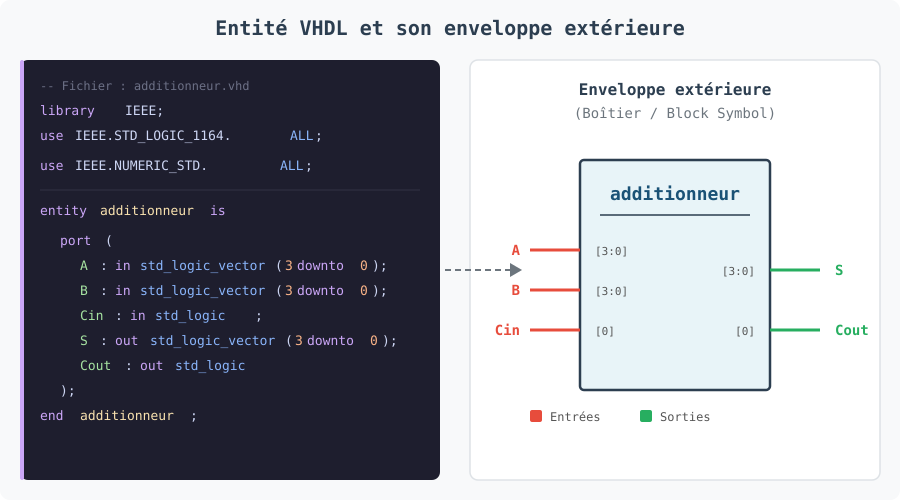
\includegraphics[scale=0.4]{./images/vhdl_entity.png}
    \end{center}
  \end{column}
\end{columns}
\end{frame}

\begin{frame}{Notion d'architecture}
  \begin{columns}

    \begin{column}{0.5\textwidth}
      \begin{alertblock}{Architecture}
        \begin{itemize}
          \item L'architecture : la vue \textbf{interne} d'un composant.
          \item Partie déclaration suivie d'un corps de l'architecture.
          \item Le corps contient des \textbf{éléments qui fonctionnent en parallèle} !
          \begin{itemize}
            \item L'ordre dans lesquels ils sont écrits est indifférent !
            \item On parle plutôt de \textbf{concurrence} (en simulation ces éléments partagent le processeur qui simule...)
          \end{itemize}
        \end{itemize}
      \end{alertblock}
    \end{column}

    \begin{column}{0.5\textwidth}
      \textbf{Eléments concurrents}
      \begin{itemize}
        \item \textbf{Assignations de signaux} : comme des équations.
        \begin{itemize}
          \item les assignations peuvent être conditionnelles ou non.
        \end{itemize}
        \item \textbf{Instanciations de composants} : assemblage hiérarchique.
        \item \textbf{Processus} : codes séquentiels isolés les uns des autres, communicants par \textit{signaux}.
      \end{itemize}
      Nous allons les passer en revue ici.
    \end{column}
  \end{columns}
\end{frame}

\begin{frame}{Architecture : notion d'\textbf{assignations concurrentes}}
  \begin{figure}[h]
    \centering
    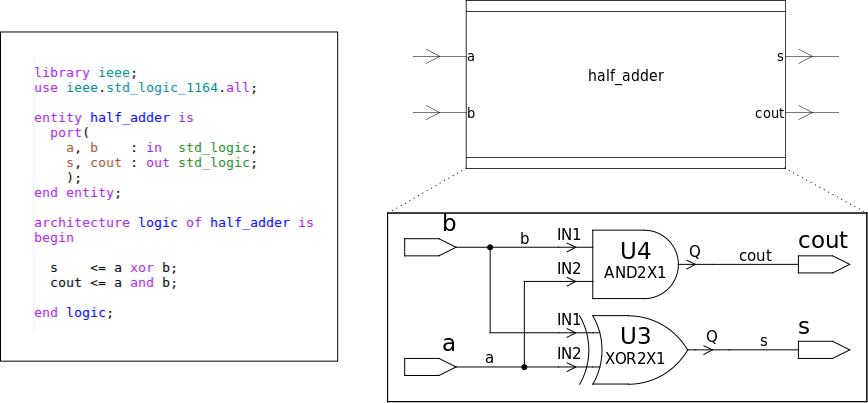
\includegraphics[scale=0.35]{./images/assignations_concurrentes.png}
  \end{figure}
\end{frame}

\begin{frame}{Architecture : notion d'\textbf{instanciation de composants}}
  \begin{figure}[h]
    \centering
    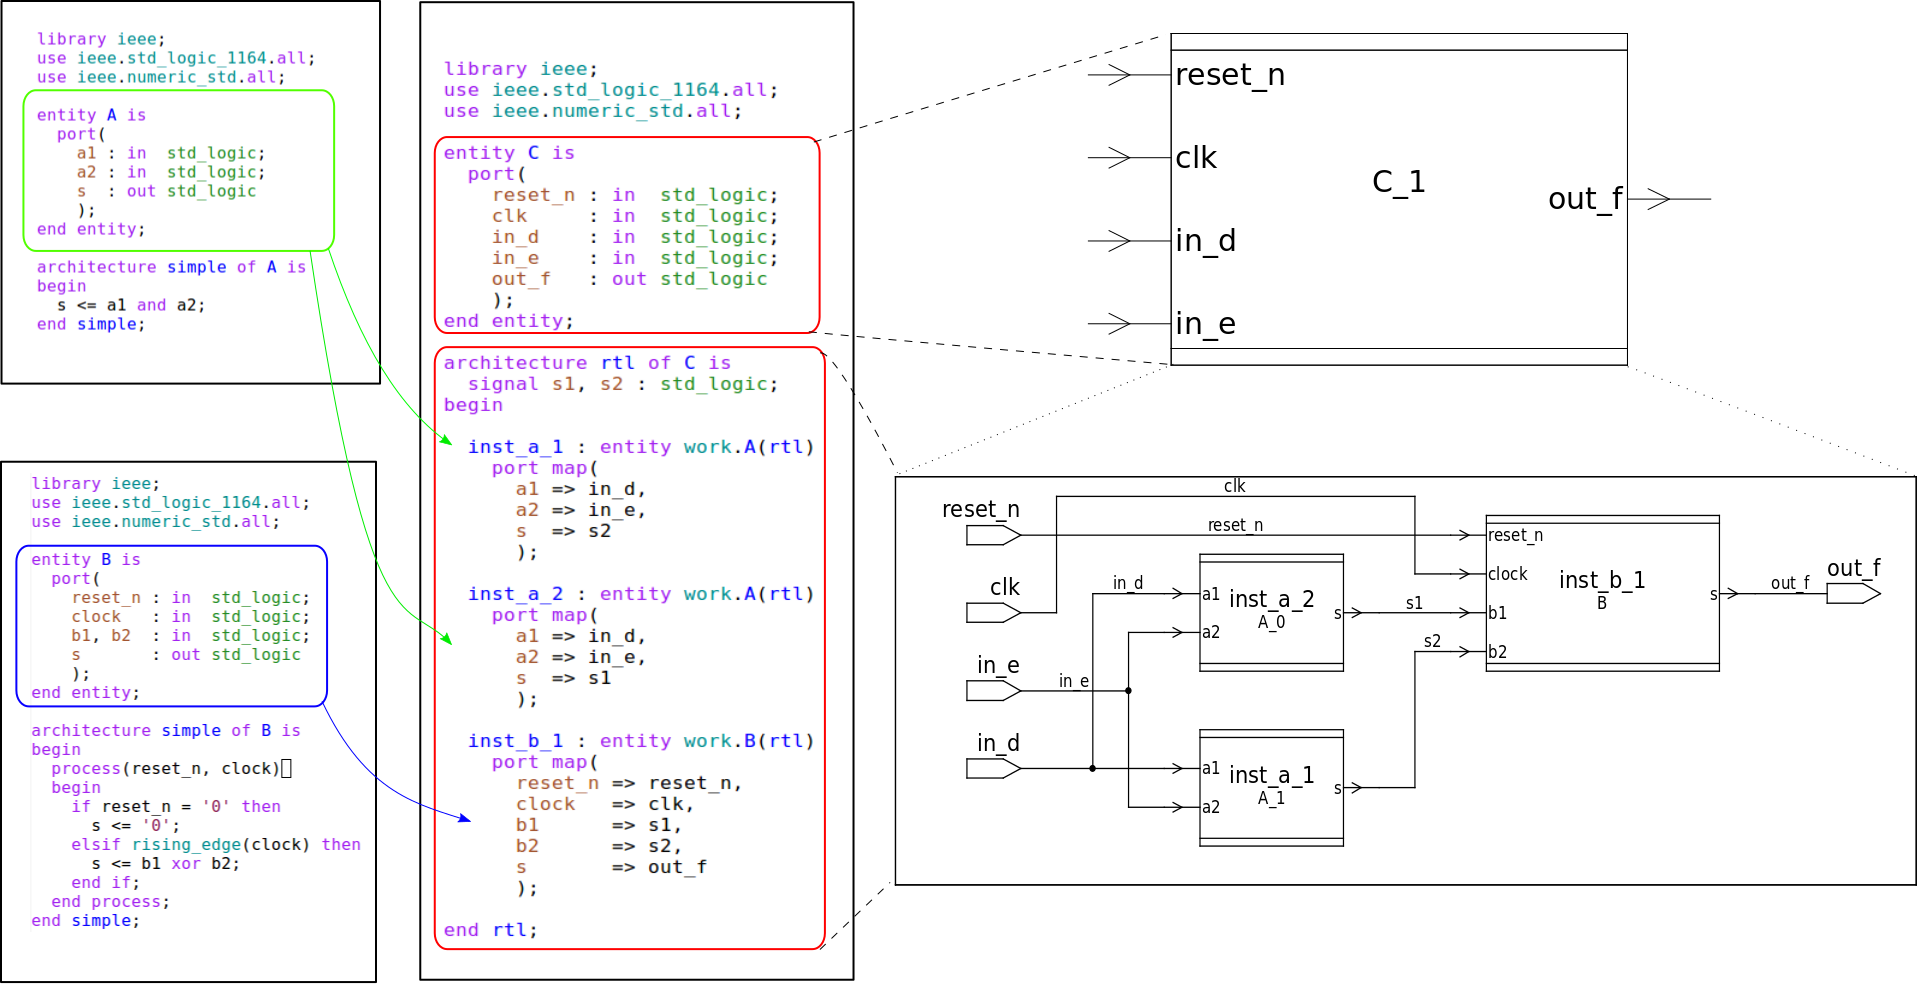
\includegraphics[scale=0.17]{./images/instanciation.png}
  \end{figure}
\end{frame}

\begin{frame}{Architecture : notion de \textbf{processus concurrents}}
  \begin{columns}
    \begin{column}{0.5\textwidth}
      \begin{itemize}
        \item Un processus est un petit programme séquentiel.
        \item Les processus fonctionnent en parallèle (concurrence).
        \item Ils communiquent par signaux.
        \item Une \textbf{liste de sensibilité} explicite permet au simulateur de savoir quand  il doit
        ré-évaluer le processus.
        \begin{itemize}
          \item observation permanente des changements de valeurs impactant le processus
        \end{itemize}
        \item Du point de vue du simulateur, les processus s'exécutent jusqu'à rencontrer un éventuel \textbf{wait}. Sinon, ils rendent la main, avant de se ré-executer.
        \item Du point de vue de la synthèse, les processus nous permettront notamment de décrire les bascules D.
      \end{itemize}
    \end{column}
    \begin{column}{0.5\textwidth}
      \begin{center}
        \includegraphics[scale=0.65]{./images/vhdl_processus.jpeg}
      \end{center}
    \end{column}
  \end{columns}
\end{frame}

\begin{frame}{Processus concurrents : exemple}
  \begin{figure}[h]
    \centering
    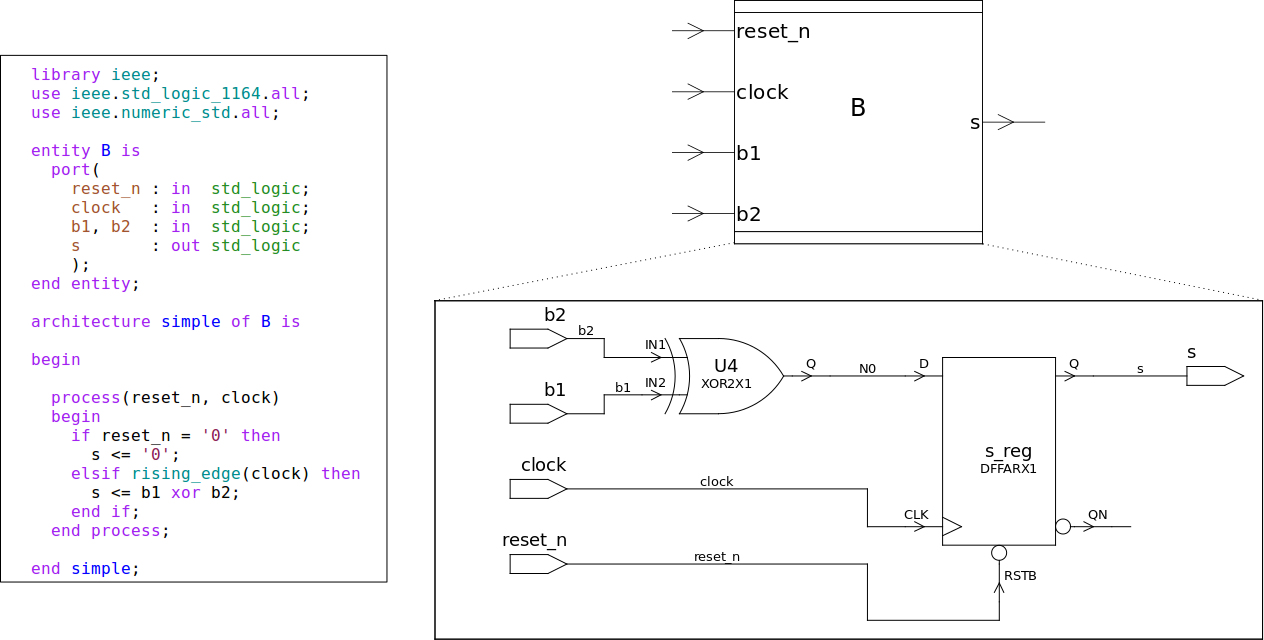
\includegraphics[scale=0.25]{./images/processus_sequentiel.png}
  \end{figure}
\end{frame}

\begin{frame}{Types en VHDL}
  On dispose de type de base, inclus dans le langage (bit par exemple), mais on repose
  plutôt sur des librairies complémentaires :
  \begin{itemize}
    \item \textbf{std\_logic\_1164} : type std\_logic, std\_logic\_vector
    \item \textbf{std\_logic} : '1','0', mais aussi 'Z','X','U','L','H'
    \begin{itemize}
      \item '0','1' : logique booléenne traditionnelle
      \item 'U' : signal 'Undefined' (non connecté)
      \item 'X' : signal en conflit. Plusieurs connexions cherchent à affecter le signal.
      \item 'Z' : haute impédance.
      \item 'L','H' : signal à peu près à '0' et '1' (peu usités)
    \end{itemize}
    \item \textbf{numeric\_std} : arithmétique traditionnelle.
    \item etc.
  \end{itemize}
  Il est possible de créer ses propres types.
  \begin{itemize}
    \item types \textbf{structurés} : \texttt{record}
    \item types \textbf{énumérés}   : \texttt{enum}
    \item types \textbf{tableaux}   : \texttt{array..of..}
  \end{itemize}
\end{frame}

\begin{frame}{Décrire des automates : en équations}
  \begin{figure}[h]
    \centering
    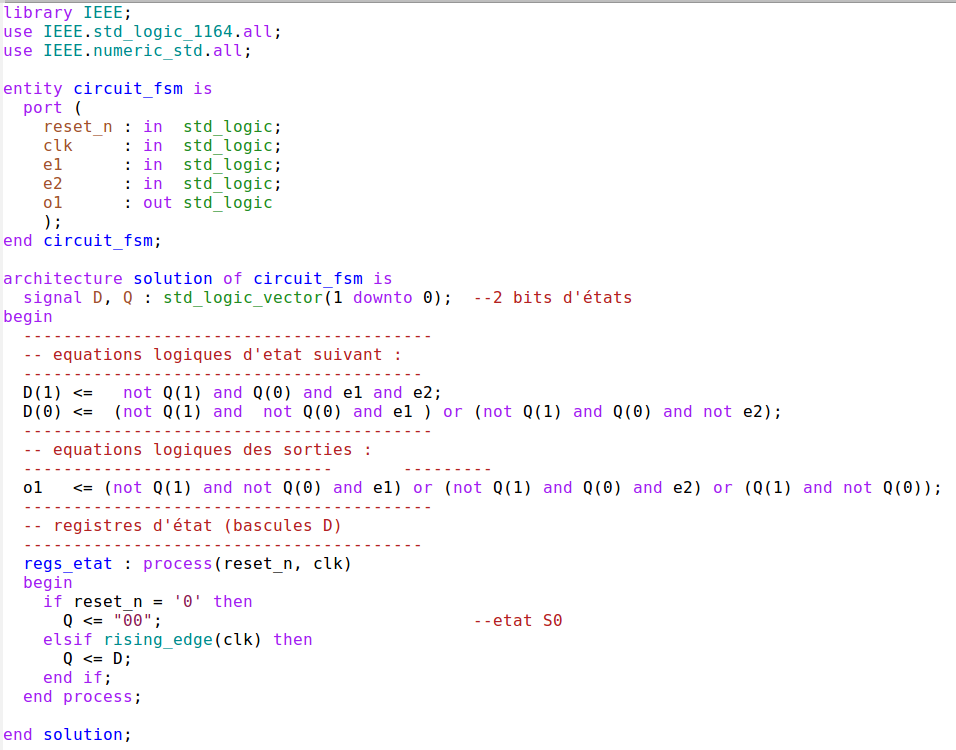
\includegraphics[scale=0.28]{./images/vhdl_1.png}
  \end{figure}
\end{frame}

\begin{frame}{Décrire des automates : en RTL}
  \begin{figure}[h]
    \centering
    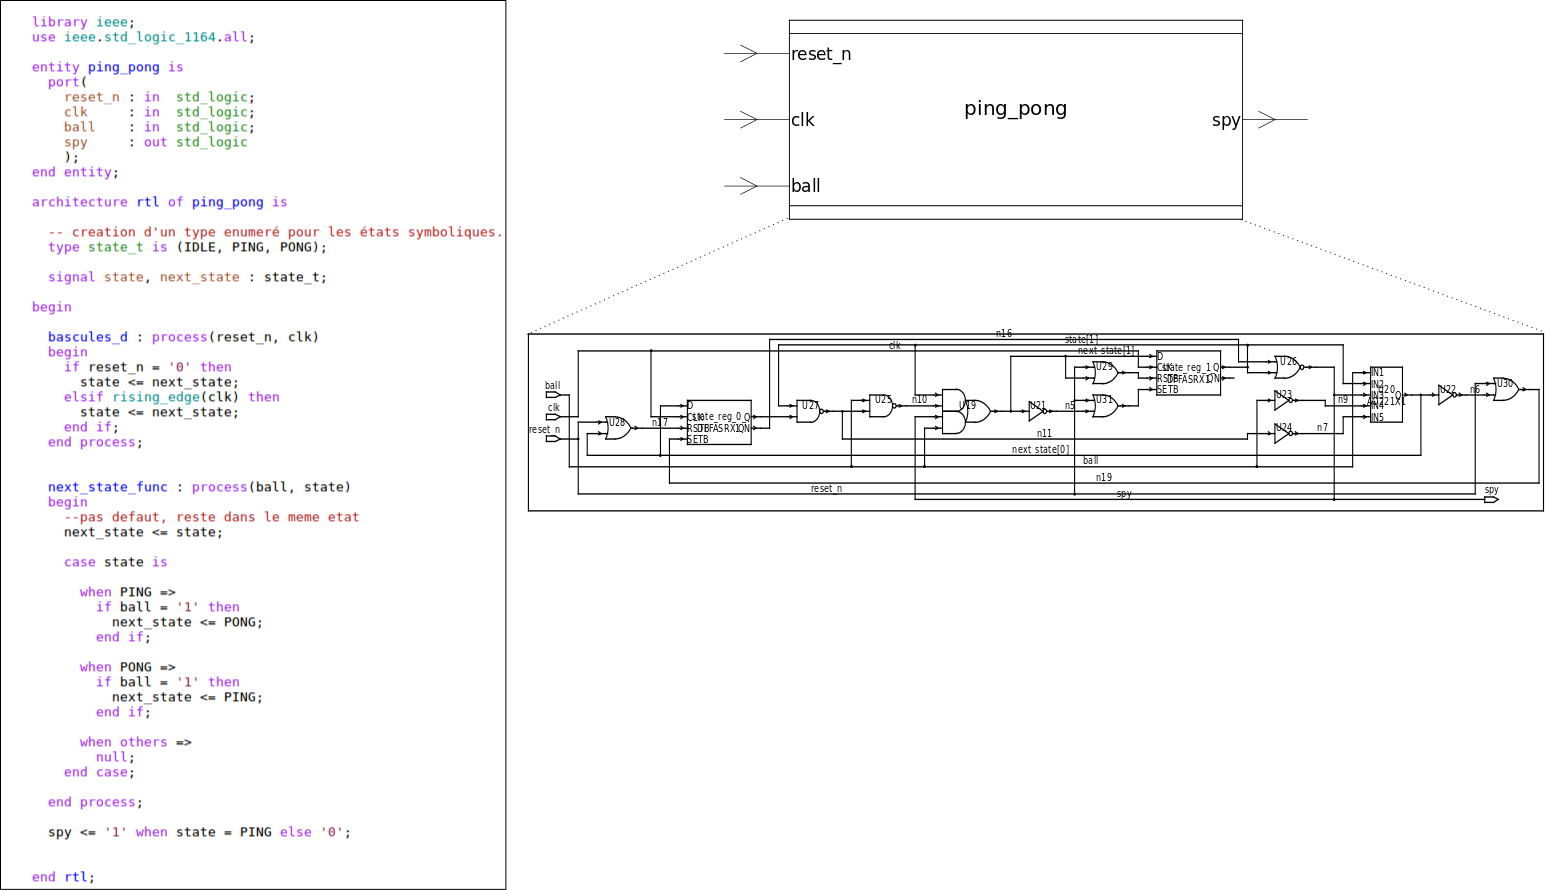
\includegraphics[scale=0.21]{./images/ping_pong_rtl.png}
  \end{figure}
  %\begin{alertblock}{Synthèse RTL}
    Le synthétiseur est capable d'\textit{inférer} les équations logiques de ce style de descriptions RTL.
  %\end{alertblock}
\end{frame}

\begin{frame}{Décrire des automates : en RTL}
  \begin{itemize}
    \item Les états sont représentés par un \textbf{type énumeré}.
    \item Deux signaux \textbf{state,next\_state} codent l'état courant et l'état futur.
    \item Un processus combinatoire permet d'expliciter le signal {\it next\_state}, à l'aide
    de différents {\it cas} présents dans le \textbf{case...when} du langage.
    \item Un processus séquentiel réalise l'échantillonnage et l'affectation de {\it next\_state} dans {\it state}
  \end{itemize}
\end{frame}

\begin{frame}{Décrire des automates : en RTL}
  \begin{itemize}
    \item A ce stade, le synthétiseur a suffisamment d'informations, pour \textbf{inférer} les équations logiques.
    \item Il a au préalable choisi un encodage de l'état. Cet encodage peut être forcé dans VHDL par des attributs ou guidés par des scripts.
    \item Le synthétiseur est capable d'explorer plusieurs solutions, notamment en fonction de l'encodage.
    \item Les sorties peuvent être encodées dans un troisème processus, mais généralement on les retrouvent dans le même processus que le calcul
    de l'état suivant.
  \end{itemize}
\end{frame}

\begin{frame}{Bancs de tests ou \textit{testbenchs}}

  \begin{columns}
    \begin{column}{0.55\textwidth}
      Les {\it testbenchs} représentent un \textbf{laboratoire virtuel} :
      \begin{itemize}
        \item le circuit à tester (DUT)
        \item des générateurs de signaux : horloge, reset, flux de données complexes.
        \item des instruments d'observations : loggers, comparateurs, etc
        \item la simulation elle-même fournit un oscilloscope, capable d'observer:
        \begin{itemize}
          \item la totalité des signaux
          \item sur une durée limitée par la seule mémoire de l'ordinateur
        \end{itemize}
      \end{itemize}

      A noter :
      \begin{itemize}
        \item seul un testbench est simulable.
        \item les bancs de test sont également décrits par un couple entité-architecture.
        \item \texttt{entity} sans port : laboratoire portes closes !
      \end{itemize}
    \end{column}
    \begin{column}{0.45\textwidth}
      \begin{center}
          \centering
          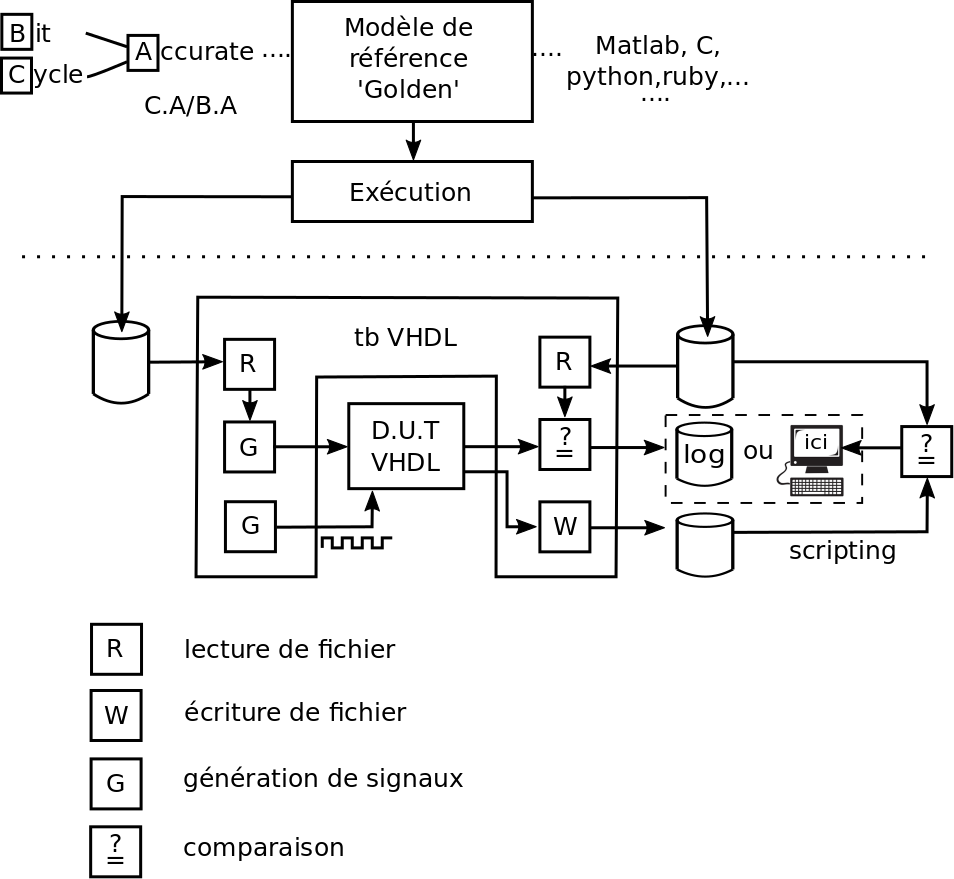
\includegraphics[scale=0.2]{./images/flot_testbench.png}
      \end{center}
    \end{column}
  \end{columns}
\end{frame}

\begin{frame}{Bancs de tests}
  \begin{itemize}
    \item Les {\it testbenchs} VHDL sont le seul moyen de tester si un circuit fonctionne correctement : un circuit seul ne fonctionne pas.
    \item Les {\it testbenchs} peuvent être de différentes natures et représentent l'essentiel du travail de concepteur.
    \begin{itemize}
      \item Testbenchs qui stimulent seulement les entrées, à partir de stimuli internes.
      \item Testbenchs qui stimulent seulement les entrées, à partir de stimuli externes (matlab, python, ruby, c, c++).
      \item Testbenchs qui vérifient les sorties, en calculant en interne les sorties attendues.
      \item Testbenchs qui vérifient les sorties, en les comparant à des valeurs calculées par un modèle externe : le \textbf{golden model}.
      \item Testbenchs qui "randomisent" la vérification, afin d'assurer une \textbf{couverture de code}.
    \end{itemize}

  \end{itemize}
\end{frame}

\begin{frame}{Banc de test VHDL : FSM \texttt{metro-boulot-dodo}}
  \begin{center}
  \begin{minipage}[t]{15cm}
   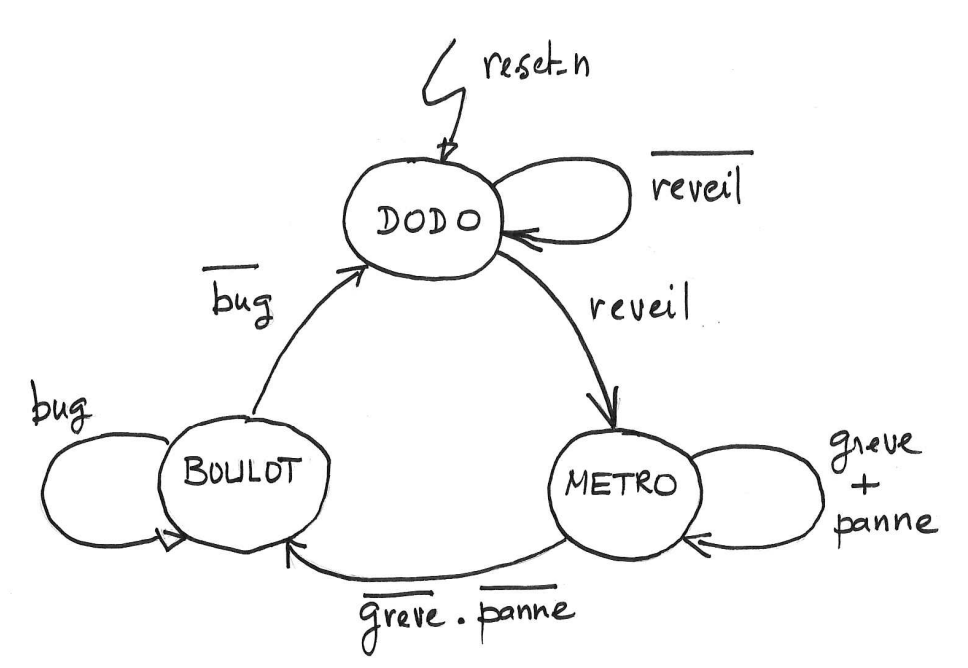
\includegraphics[width=10cm]{./images/iloveparis.png}
  \end{minipage}
  \end{center}
\end{frame}

\begin{frame}{Banc de test VHDL : exemple}
  \begin{center}
   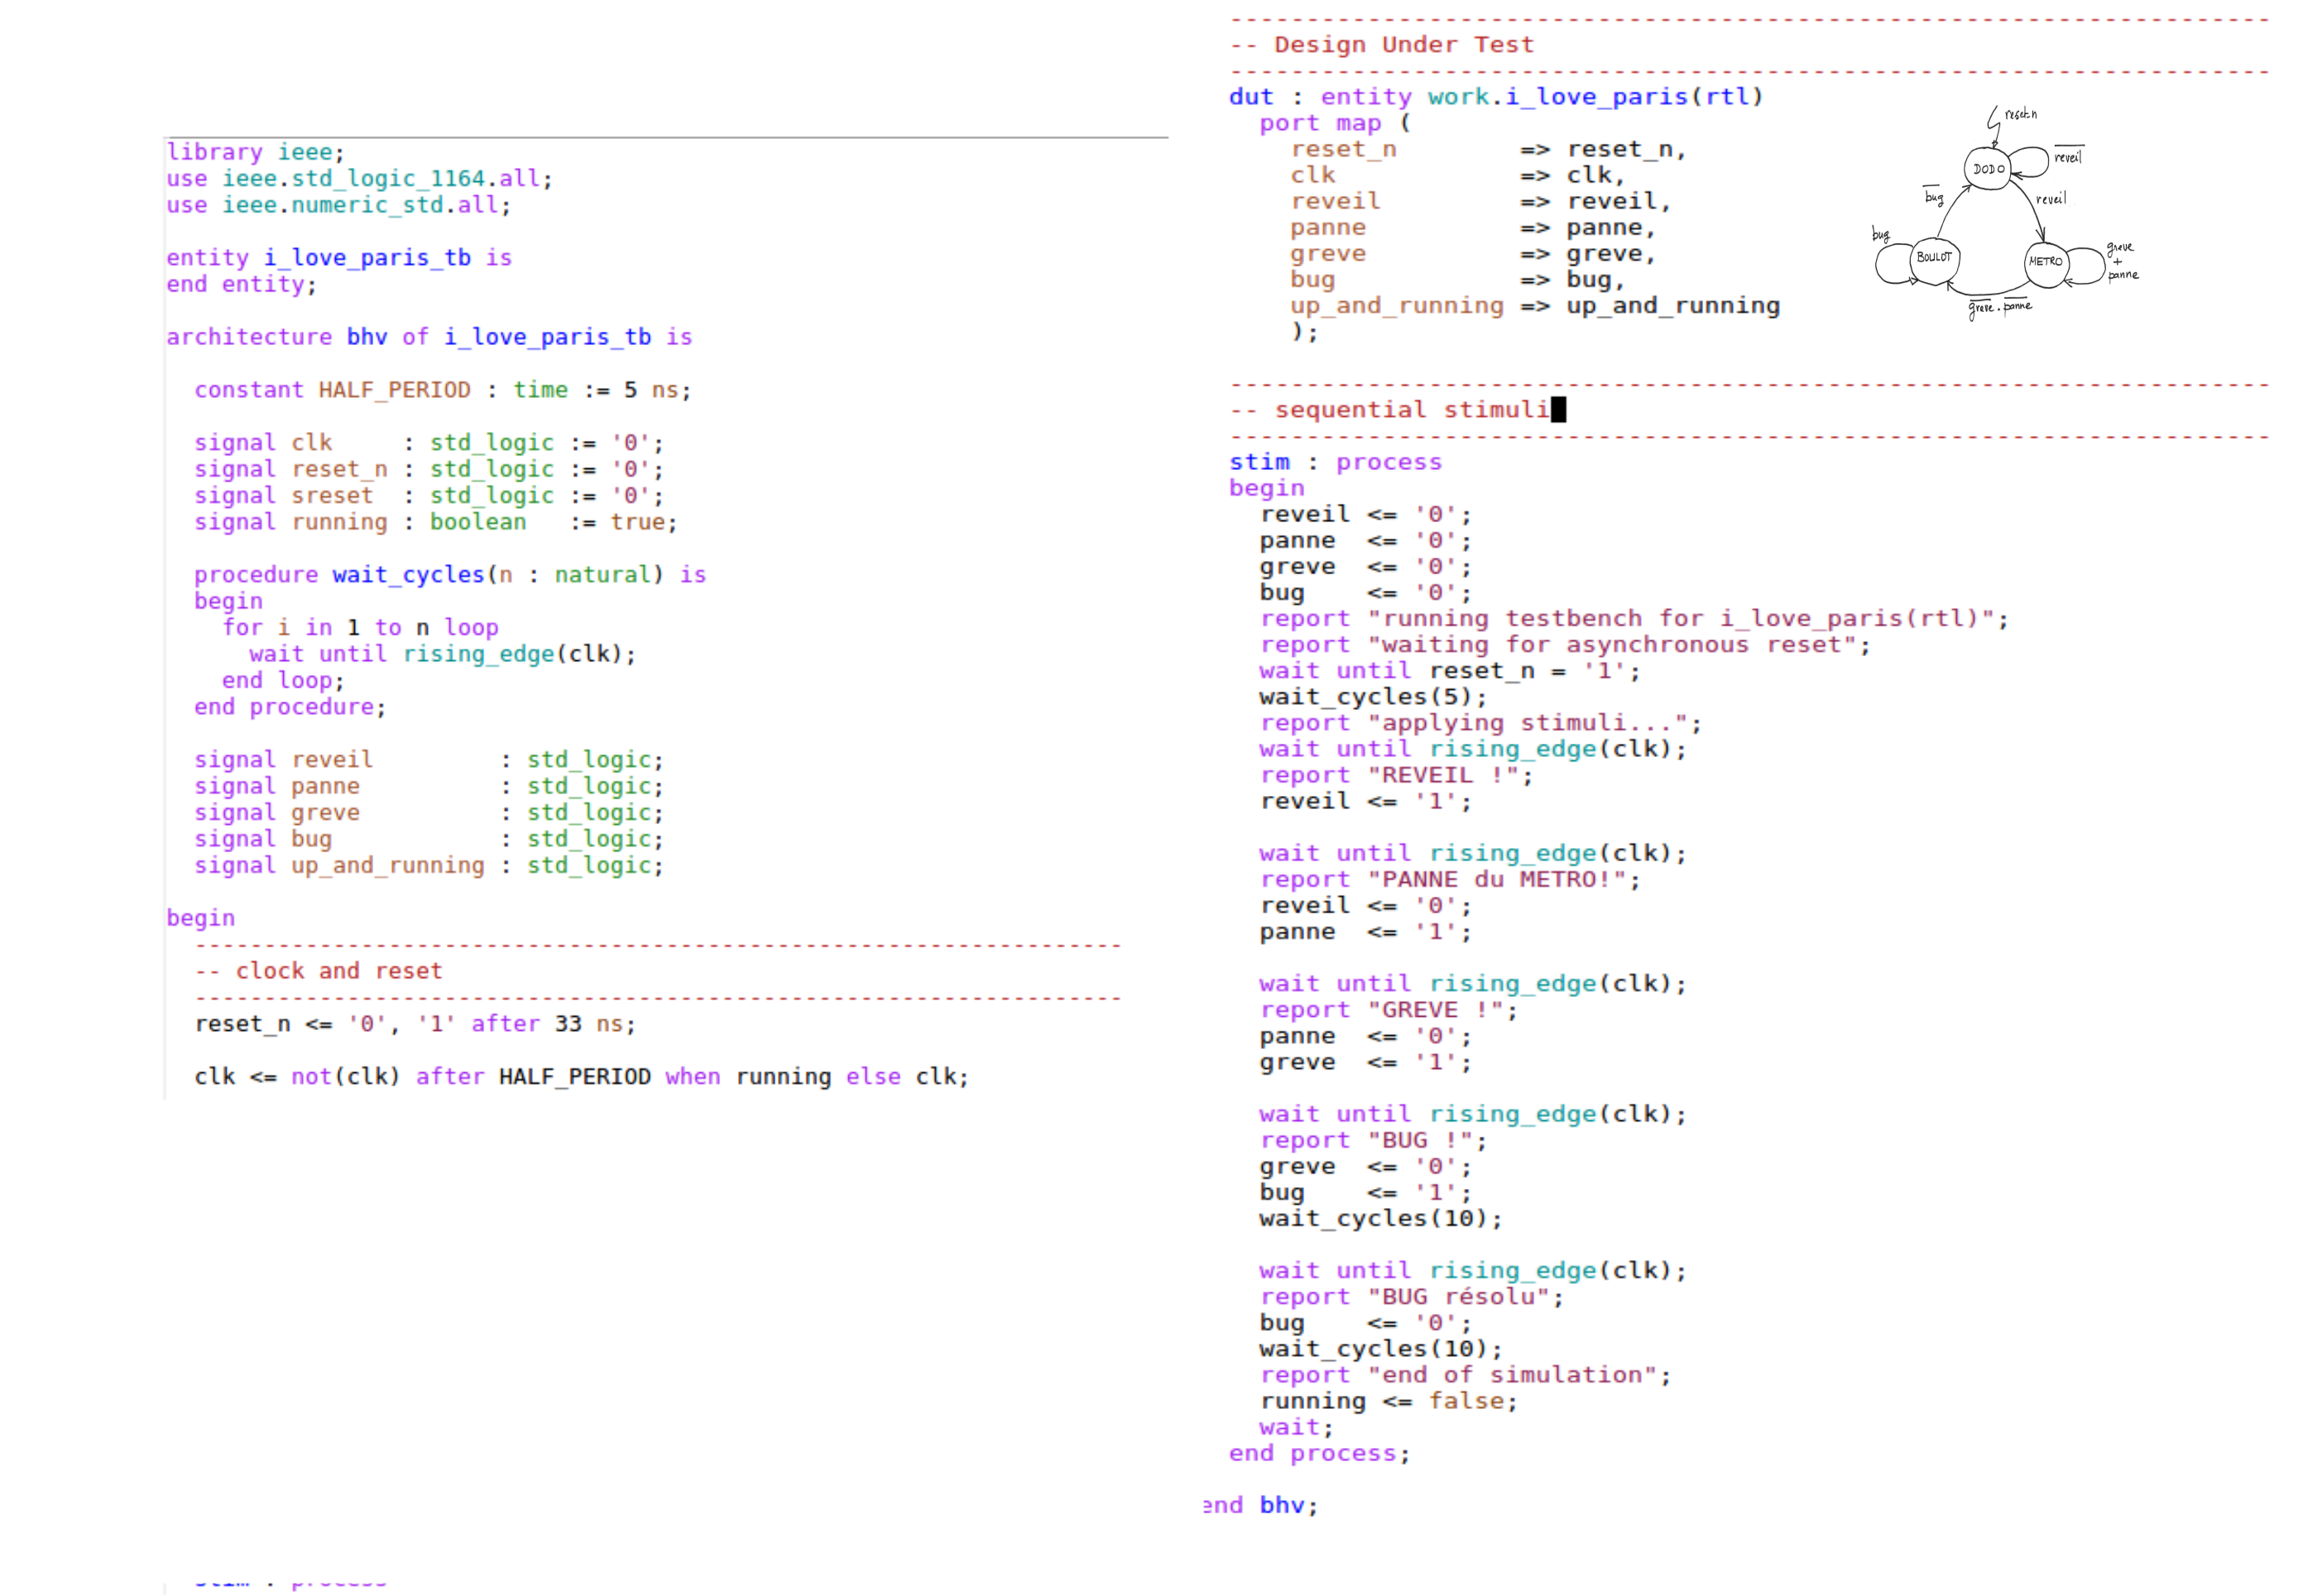
\includegraphics[scale=0.12]{./images/tb_000.png}
  \end{center}
\end{frame}

\begin{frame}{Banc de test VHDL : exemple}
  \begin{center}
   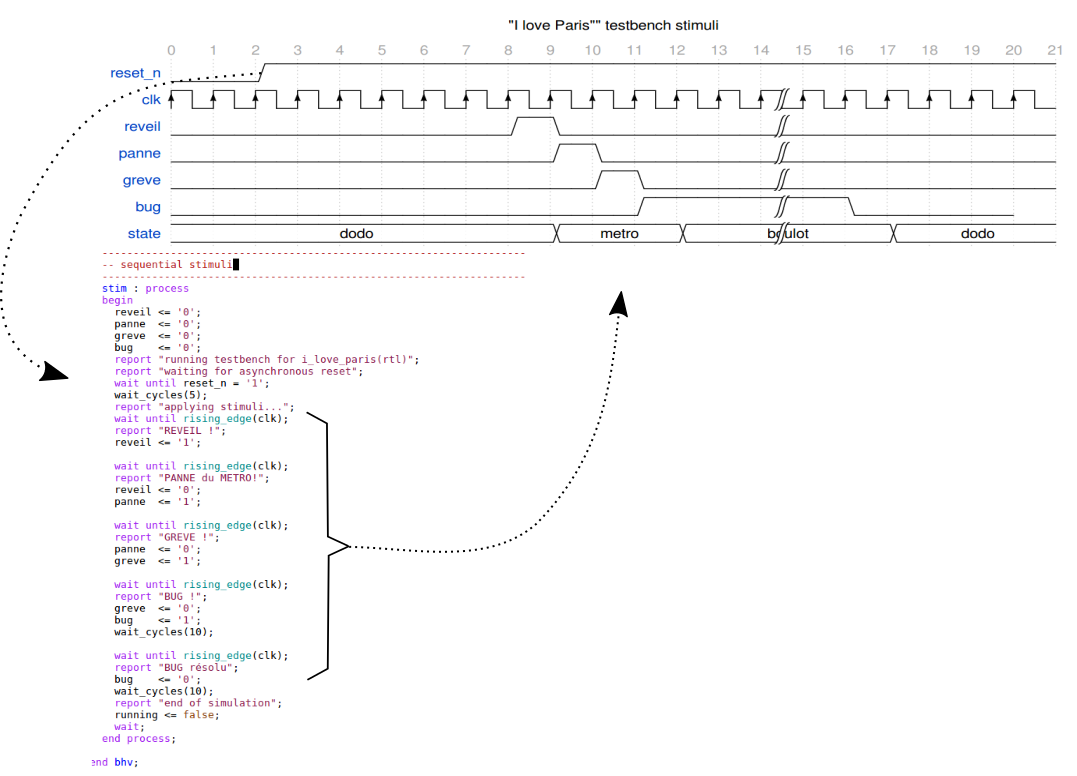
\includegraphics[scale=0.28]{./images/wave_drom.png}
  \end{center}
\end{frame}

\begin{frame}{Pour la petite histoire...}
  Les {\it timing diagrams} ont été crées avec une syntaxe textuelle ! Le compilateur
  transforme ces {\it timing diagrams} en graphique SVG dans html5.
  \begin{center}
  \begin{minipage}[t]{19cm}
   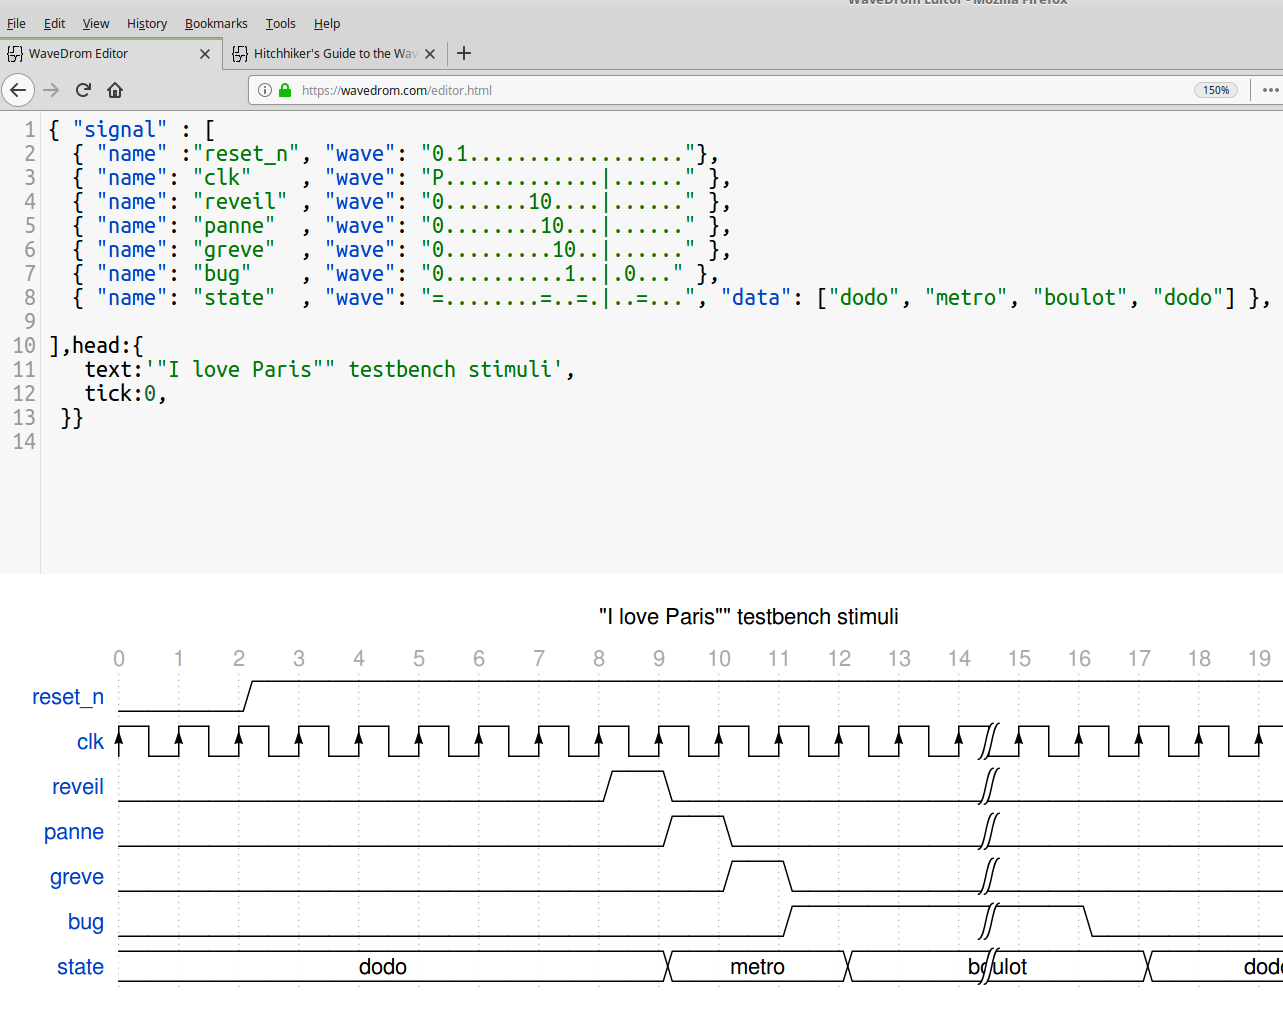
\includegraphics[scale=0.17]{./images/wave_drom_ex.png}
  \end{minipage}
  \end{center}
\end{frame}

\begin{frame}{Banc de test VHDL : exemple}
  Chronogrammes issus de la chaîne de compilation-simulation-visualisation autour de GHDL+Gtkwave.
  \begin{center}
  \begin{minipage}[t]{19cm}
   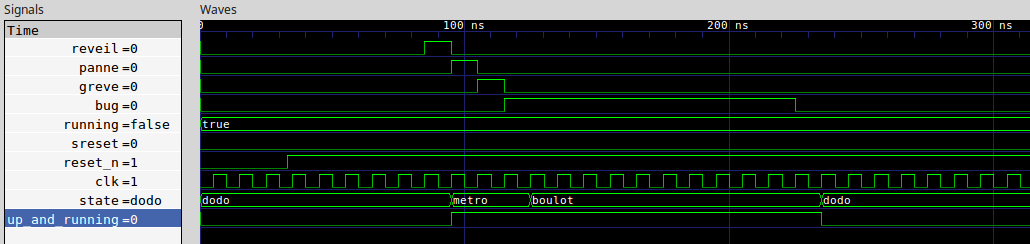
\includegraphics[scale=0.32]{./images/metro_boulot_dodo_chrono.png}
  \end{minipage}
  \end{center}
\end{frame}

\begin{frame}{Simulation avec GHDL ou NVC}
  \begin{columns}
    \begin{column}{0.5\textwidth}
      \texttt{GHDL} est un simulateur et synthétiseur open source développé par un français : Tristan Gingold.
      \begin{itemize}
        \item Il est open source. Développé en ADA.
        \item Il supporte les évolutions récentes du langage.
        \item Il est scrupuleux sur le respect de la norme.
        \item On peut le coupler à \texttt{gtkwave} pour l'examen des signaux.
        \item Ce n'est pas le simulateur le plus utilisé au Monde : il s'agit de Modelsim.
      \end{itemize}
      \texttt{NVC} est un autre simulateur (pas de synthèse) open source développé par un brittanique : Nick Gasson.
    \end{column}
    \begin{column}{0.5\textwidth}
      \begin{center}
        \begin{figure}
          \includegraphics[scale=0.2]{./images/Tristan_Gingold.jpg}
          \caption{Tristan Gingold, ingénieur de Recherche au \texttt{C.E.R.N}, Génève (Telecom Paris 96, DEA Microélectronique (Paris 6) 98.)}
        \end{figure}
      \end{center}
    \end{column}
  \end{columns}
\end{frame}

\begin{frame}{Simulation avec GHDL}
  Pour simuler un testbench, il faut passer par 3 phases :
  \begin{itemize}
    \item \textbf{A}nalyse : \textbf{ ghdl -a circuit.vhd}
    \item ...
    \item \textbf{A}nalyse : \textbf{ghdl -a circuit\_tb.vhd}
    \item \textbf{E}laboration : \textbf{ghdl -e circuit\_tb} (sans .vhd).
    \begin{itemize}
      \item cette phase réunit les fichiers binaires produits par l'analyse
      \item ...adjoint un {\it runtime} (le coeur du simulateur)
      \item ...et produit un exécutable : le simulateur
    \end{itemize}
    \item \textbf{R}un : \textbf{ghdl -r circuit\_tb --wave=waves.ghw}.
    \begin{itemize}
      \item Le simulateur s'exécute et enregistre les signaux dans le fichier waves.
    \end{itemize}
    \item Un viewer externe est alors utilisé pour visualiser les signaux : \textbf{gtkwave waves.ghw}.
    \item La disposition des signaux est enregistrable dans un fichier spécifique à gtkwave (.sav).
    \item Il faut \textbf{scripter} l'ensemble.
  \end{itemize}
\end{frame}

\begin{frame}{Visualisation avec Gtkwave}
  \textbf{gtkwave wave.ghw chrono.sav}
  Le fichier chrono.sav correspond à la mise en forme des chronogrammes, sauvée dans ce fichier.
  \begin{center}
  \begin{minipage}[t]{8cm}
   \centering
   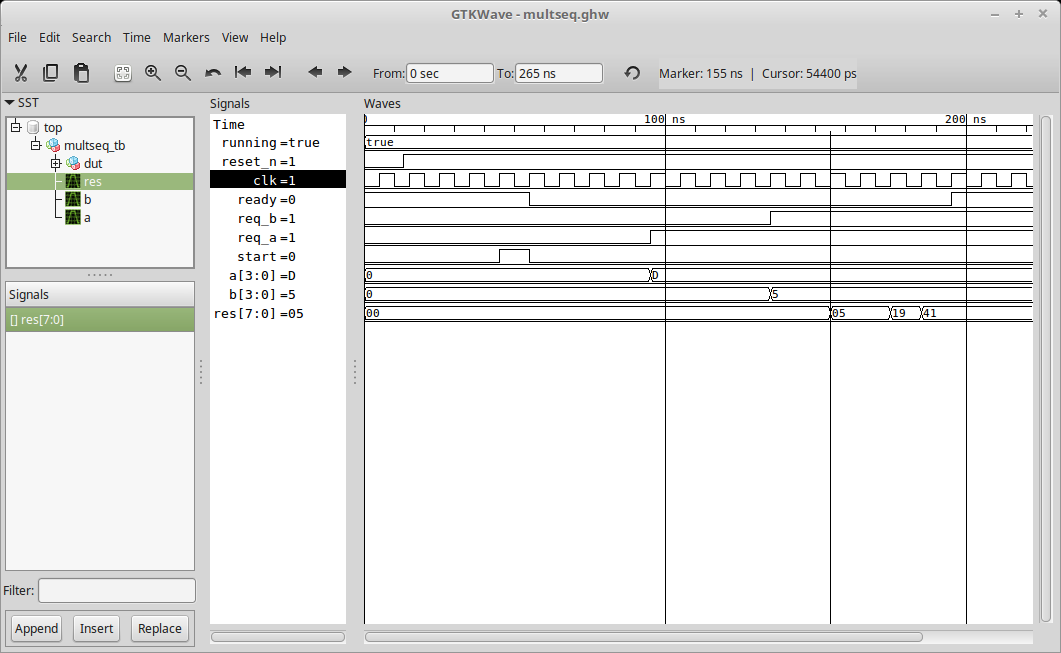
\includegraphics[width=8cm]{./images/gtkwave.png}
  \end{minipage}
  \end{center}
\end{frame}
